\documentclass[11pt,xcolor={svgnames},aspectratio=169,usepdftitle=false]{beamer}

%===========================================================
% DOCUMENT
%===========================================================
\usepackage{rafa_style_beamer}
\addbibresource{../matlab_intro.bib}
\title{Introduction to Matlab}
\subtitle{Lesson 04 --- Optimization}

\author{Rafael Serrano-Quintero}

\institute{Department of Economics \\ University of Barcelona}
\date{}

\begin{document}

\VerbatimFootnotes

\maketitle

\section{Optimization Preliminaries}

\begin{frame}
  \frametitle{Optimization Preliminaries}
\begin{itemize}
  \item \alert{\textbf{Agents optimize}} is the foundational assumption of economic theory.
  \begin{itemize}
    \item Firms minimize costs / maximize profits.
    \item Consumers maximize utility / minimize expenditures.
  \end{itemize}
  \item Not only in theory \ldots Econometricians use
  \begin{itemize}
    \item Maximum likelihood, least squares, method of moments \ldots
    \item All optimization problems.
  \end{itemize}
  \item We will learn the basics of how to state and solve this type of problems in Matlab.
\end{itemize}
\end{frame}

\begin{frame}
  \frametitle{Optimization Preliminaries --- Definition of the Problem}
The most general definition of an optimization problem
\begin{align}
  \underset{x\in\mathbb{R}^n}{\min} \phantom{\Omega} &   f(x) \tag{Objective Function} \label{eqn:objective_func} \\
  \text{s.t. } & g(x) = 0 \tag{Equality Constraints} \label{eqn:equality_constr} \\
  \phantom{\text{s.t.}} & h(x) \leq 0 \tag{Inequality Constraints} \label{eqn:inequality_constr}
\end{align}
where
\begin{itemize}
  \item the \ref{eqn:objective_func} $f :\mathbb{R}^n\mapsto \mathbb{R}$
  \item the $m$ \ref{eqn:equality_constr} $g :\mathbb{R}^n\mapsto \mathbb{R}^m$
  \item the $l$ \ref{eqn:inequality_constr} $h :\mathbb{R}^n\mapsto \mathbb{R}^l$
\end{itemize}
\end{frame}

\begin{frame}
  \frametitle{Optimization Preliminaries --- Definitions}
Let $f : \mathcal{D}\subseteq\mathbb{R}^n \mapsto \mathbb{R}$. 

\begin{definition}
A \alert{\textbf{critical point}} $x^*\in\mathcal{D}$ of $f$ satisfies $\nabla f(x^*) \equiv \left(\dfrac{\partial f}{\partial x_1}(x^*), \ldots,\dfrac{\partial f}{\partial x_n}(x^*)\right) = 0$.
\end{definition}

\begin{definition}
A point $x^*\in\mathcal{D}$ is a \alert{\textbf{min}} of $f$ on $\mathcal{D}$ if $f(x^*)\leq f(x) \forall x\in\mathcal{D}$. It is a \alert{\textbf{strict min}} if $f(x^*) < f(x) \forall x\neq x^*\in\mathcal{D}$.
\end{definition}

\begin{definition}
A point $x^*\in\mathcal{D}$ is a \alert{\textbf{local (or relative or weak) min}} of $f$ on $\mathcal{D}$ if there is a ball $B_r(x^*)$ such that $f(x^*) \leq f(x) \forall x\in B_r(x^*)\cap\mathcal{D}$. It is a \alert{\textbf{strict local (or relative or weak) min}} if $f(x^*) < f(x) \forall x\neq x^*\in B_r(x^*)\cap\mathcal{D}$
\end{definition}
\end{frame}

\begin{frame}
  \frametitle{Optimization Preliminaries --- Definitions}
\begin{figure}
  \centering
    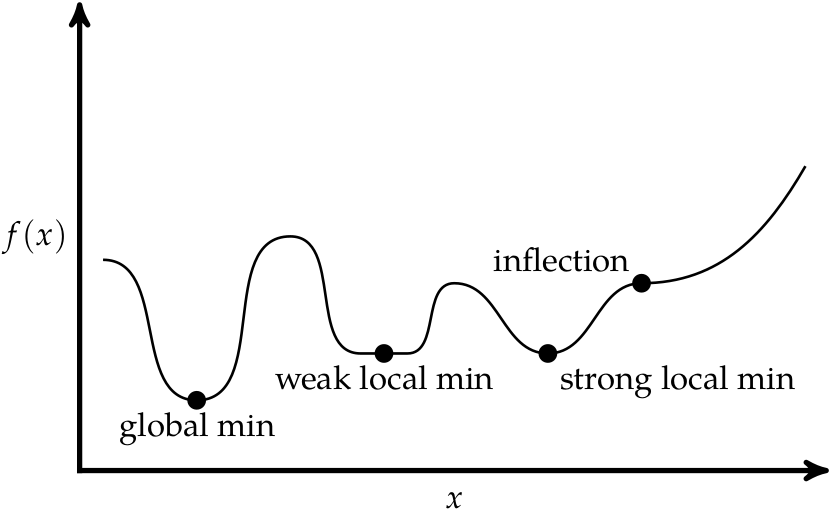
\includegraphics[width = 0.75\textwidth]{../figures/classification_critical_points.png}
    \caption{Classification of Critical Points. See \cite{kochenderfer2019optimization}}
\end{figure}
\end{frame}

\begin{frame}
  \frametitle{Optimization Preliminaries --- First Order Conditions}
\begin{itemize}
  \item All points \alert{\textbf{need}} that $f'(x^*) = 0$. Notice this is a \alert{\textbf{necessary condition}} but not sufficient.
  \item The inflection point also has $f'(x^*) = 0$ {\tiny (An inflection point is where the sign of the second derivative changes)}.
\end{itemize}

\begin{theorem}
Let $f : \mathcal{D}\subseteq\mathbb{R}^n \mapsto \mathbb{R}$ be a $\mathcal{C}^1$ function. If $x^*$ is a local min or max of $f$ in $\mathcal{D}$ and $x^*$ is an interior point of $\mathcal{D}$, then
\[
\nabla f(x^*) = 0 \ \text{ for } i = 1,\ldots, n
\]
\end{theorem}
\end{frame}

\begin{frame}
  \frametitle{Optimization Preliminaries --- Second Order Conditions}
\begin{theorem}
Let $f : \mathcal{D}\subseteq\mathbb{R}^n \mapsto \mathbb{R}$ be a $\mathcal{C}^2$ function. Suppose $x^*$ is a critical point of $f$.
\begin{enumerate}
  \item If $H_f(x)$ is positive (negative) definite, then $x^*$ is a strict local min (max) of $f$.
  \item If $H_f(x)$ is indefinite, then $x^*$ is neither a local min or max of $f$.
\end{enumerate}
\end{theorem}

\begin{definition}
Let $f : \mathcal{D}\subseteq\mathbb{R}^n \mapsto \mathbb{R}$ be a $\mathcal{C}^2$ function. The Hessian matrix $H_f$ is a square $n\times n$ matrix whose $(i,j)-$th entry is defined by $(H_f)_{i,j} = \dfrac{\partial^2 f}{\partial x_i \partial x_j}$.
\end{definition}
\end{frame}

\begin{frame}
  \frametitle{Optimization Preliminaries --- Recap}
\begin{itemize}
  \item This has been a very brief recap on basic optimization.
  \item For a refresher, you can take a look at \cite[Chapters~17-19]{simon1994mathematics}.
  \item We will cover the very basics of optimization and implementation in Matlab.
  \item All numerical optimization methods:
  \begin{itemize}
    \item Search for \alert{\textbf{feasible choices}}
    \item Generate a sequence of \alert{\textbf{guesses}}
    \item Try to make the sequence \alert{\textbf{converge}} to the true solution.
  \end{itemize}
  {\tiny Pretty similar to root finding algorithms\ldots right?}
\end{itemize}
\end{frame}

\section{Optimization in One Dimension}

\begin{frame}
  \frametitle{The Simplest Optimization Problem}

The simplest optimization problem is \alert{\textbf{unconstrained optimization}} in one dimension
\[
\underset{x\in\mathbb{R}}{\min} \phantom{\Omega} f(x)
\]
where $f : \mathbb{R}\mapsto\mathbb{R}$.
Why focusing on one dimension?
\begin{enumerate}
  \item Illustrate techniques in a clear way.
  \item Many multivariate methods boil down to solving a sequence of one-dimensional problems.
\end{enumerate}
\end{frame}

\begin{frame}
  \frametitle{Optimization Methods --- Categories}
Four general categories for optimization methods:
\begin{enumerate}
  \item Use derivatives.
  \item Do not use derivatives.
  \item Mixed methods.
  \item Simulation-based methods.
\end{enumerate}

We will look at methods in the first two.
\end{frame}

\subsection{Bracketing Method}

\begin{frame}
  \frametitle{Bracketing Method --- The Intuition}
  \begin{columns}
  \begin{column}{0.49\textwidth}
    \begin{itemize}
      \item Suppose $f : \mathbb{R}\mapsto\mathbb{R}$ is \href{https://en.wikipedia.org/wiki/Unimodality\#Unimodal_function}{unimodal}.
      \item Let $a<b<c\in\mathbb{R}$ be three points such that
      \begin{equation}
        f(a), f(c) > f(b) \label{eqn:bracketing_criterion}
      \end{equation}
      \item Then, we know a minimum exists in $[a,c]$.
      \item How to find the optimum?
    \end{itemize}
  \end{column}
  \begin{column}{0.5\textwidth}
    \begin{figure}
      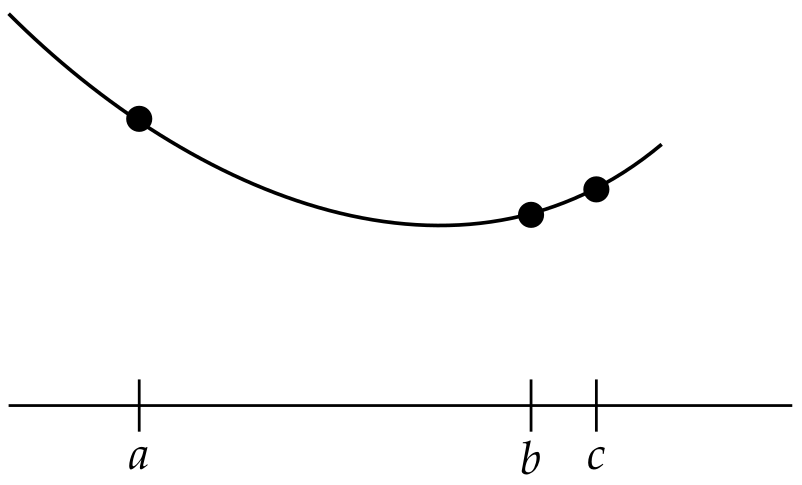
\includegraphics[width=0.95\textwidth]{../figures/optimization_bracketing.png}
      \caption{See \cite{kochenderfer2019optimization}}
    \end{figure}
  \end{column}
\end{columns}
\end{frame}

\begin{frame}
  \frametitle{Bracketing Method --- The Algorithm}
\begin{enumerate}
  \item Define $h$ as the step size, a constant $\alpha > 1$, and a given initial $x_0$ and compute
  \[
  f(x_0), f(x_0 \pm \alpha h), f(x_0 \pm \alpha^2 h), \ldots
  \]
  until we find a triplet satisfying \eqref{eqn:bracketing_criterion}. Choose a stopping criterion $\varepsilon$.
  \item If $b - a < c - b$, set $d = (b+c)/2$, otherwise, $d = (a+b) / 2$. Compute $f(d)$.
  \item If $d < b$ and $f(d) > f(b)$, replace $(a,b,c)$ with $(d,b,c)$. If $d<b$ and $f(d) < f(b)$, replace $(a,b,c)$ with $(a,d,b)$. If $d > b$ and $f(d) < f(b)$, replace $(a,b,c)$ with $(b,d,c)$.  Otherwise, replace $(a,b,c)$ with $(a,b,d)$.
  \item If $c - a < \varepsilon$, stop. Otherwise, go to step 2.
\end{enumerate}
\end{frame}

\begin{frame}
  \frametitle{Bracketing Method --- Remarks}
\begin{itemize}
  \item Slow. Similar to bisection.
  \item The stopping criterion is clear. If the length of the interval $[a,c]$ is sufficiently small, for practical terms, we have found the optimum.
  \item The method finds a \alert{\textbf{local minimum}}, depending on the starting triplet $(a,b,c)$ the method will converge to one minimum or another. {\tiny This is a fairly common problem in many methods.}
  \item If we know there is only one solution, the method always converges.
  \item Note we need three points in each iteration, depending on how costly it is to compute $f$ this might be a problem.
\end{itemize}
\end{frame}

\begin{frame}
  \frametitle{Bracketing Method --- An Example}
Let's minimize
\[
f(x) = \frac{x^2}{2} - x
\]
\begin{itemize}
  \item The function has a global minimum in $x = 1$.
  \item Let us divide the code into two blocks:
  \begin{enumerate}
    \item Initial bracketing.
    \item Refining given the bracketing.
  \end{enumerate}
\end{itemize}
\end{frame}

\begin{frame}
  \frametitle{Bracketing Method --- Initial Bracketing}
\begin{enumerate}
  \item Start from guess $x_0$ and compute $x_1 = x_0 + \alpha h$.
  \item Evaluate $f(x_0)$ and $f(x_1)$. If $f(x_1) < f(x_0)$ keep increasing until $f(x_2) > f(x_1)$
  \item Otherwise, change direction and increase interval until $f(x_2) > f(x_0)$.
  \item Increase $\alpha$ in each step to make the interval larger.
\end{enumerate}
\end{frame}

\begin{frame}[fragile]
  \frametitle{Bracketing Method --- Initial Bracketing}
\begin{itemize}
  \item Start from guess $x_0 = -5$ {\tiny (why not?)} and compute increment.
  \begin{lstlisting}
  % Parameters of bracketing method
  h = 1e-2;
  alp = 1.1;
    
  % Step 1 - Initial bracketing
  x0 = -5;
  fx0 = fun(x0);
  x1 = x0 + alp*h;
  fx1 = fun(x1);
  % If function is increasing in this direction, change direction  
  if fx1 > fx0
      h = -h;
  end
  \end{lstlisting}
\end{itemize}
\end{frame}

\begin{frame}[fragile]
  \frametitle{Bracketing Method --- Initial Bracketing}
\begin{itemize}
  \item Stablish the outer loop.
  \begin{lstlisting}
  condition = true;
  it = 1;
  while condition
  % Outer loop
  end
  \end{lstlisting}
  \item Suppose $h < 0$
  \begin{lstlisting}
  x2 = x0 + alp*h; 
  fx2 = fun(x2);
  % We found the function increases!
  if fx2 > fx0
    a = x2;
    b = x0;
    c = x1;
    condition = false;
  end
  \end{lstlisting}
\end{itemize}
\end{frame}

\begin{frame}[fragile]
  \frametitle{Bracketing Method --- Initial Bracketing}
\begin{itemize}
  \item Suppose $h > 0$
  \begin{lstlisting}
  x2 = x1 + alp*h;
  fx2 = fun(x2);
  % We found the function increases!
  if fx2 > fx1
    a = x0;
    b = x1;
    c = x2;
    condition = false;
  end
  \end{lstlisting}
  \item If we have not found the function increases, update $\alpha$
  \begin{lstlisting}
  alp = alp*2;
  \end{lstlisting}
  \item Then, simply put all together in nested \verb;if-else; statements.
\end{itemize}
\end{frame}

\begin{frame}[fragile]
  \frametitle{Bracketing Method --- Refining Bracketing}
\begin{itemize}
  \item Initiallize loop
  \begin{lstlisting}
  while (difference > tol) && (it < maxit)
      % Stuff goes here
  end
  \end{lstlisting}
  \item Define $d$ and compute $f(d)$
  \begin{lstlisting}
  % Step 2: define d and compute f(d)
  if (b - a) > (c - b)
      d = (a + b)/2;
  else
      d = (b + c)/2;
  end
  fd = fun(d);
  \end{lstlisting}
\end{itemize}
\end{frame}

\begin{frame}[fragile]
  \frametitle{Bracketing Method --- Refining Bracketing}
\begin{minipage}{0.48\textwidth}
  \begin{itemize}
    \item Refine the interval if $d < b$
    \begin{lstlisting}
% Step 3: refine the interval
if d < b
    if fd > fb
        a1 = d;
        b1 = b;
        c1 = c;
    else
        a1 = a;
        b1 = d;
        c1 = b;
    end
else
    \end{lstlisting}
  \end{itemize}
\end{minipage}
\begin{minipage}{0.48\textwidth}
  \begin{itemize}
    \item Refine the interval if $d > b$
    \begin{lstlisting}
% Step 3: refine the interval
else
  if fb < fd
      a1 = a;
      b1 = b;
      c1 = d;
  else
      a1 = b;
      b1 = d;
      c1 = c;
  end
end
    \end{lstlisting}
  \end{itemize}
\end{minipage}
Rename \verb;a1; by \verb;a;, compute $(c - a)$, and update iteration counter.
\end{frame}

\subsection{Newton-Raphson Method}

\begin{frame}
  \frametitle{Newton-Raphson Method}
\begin{itemize}
  \item Familiar? Yes! It is very closely related to the root finding algorithm!
  \item Given an initial $x_0$, compute a second order Taylor expansion around $x_0$:
  \[
  f(x) \approx f(x_0) + f'(x_0)(x - x_0) + \frac{f''(x_0)}{2}(x - x_0)^2
  \]
  \item Minimizing this approximation, the FOC we get is
  \[
  f'(x_0) + f''(x_0)(x^* - x_0) = 0
  \]
  solving for $x^*$
  \[
  x^* = x_0 - \frac{f'(x_0)}{f''(x_0)}
  \]
  \item Which is the \alert{\textbf{same iteration scheme}} that we saw previously!
\end{itemize}
\end{frame}

\begin{frame}
  \frametitle{Newton-Raphson Method --- Remarks}
\begin{itemize}
  \item Newton-Raphson's method tries to finds \alert{\textbf{critical points}}.
  \item We \alert{\textbf{must check}} $f''(x^*)$ to check what we have found.
  \item Problems:
  \begin{itemize}
    \item Convergence is not ensured.
    \item $f''(x)$ might be difficult to compute. If we rely on finite difference methods, we will be adding errors.
    \item Very sensitive to initial conditions.
  \end{itemize}
  \item \href{https://www.sas.upenn.edu/~jesusfv/Lecture_NM_2_Optimization.pdf}{From Fern\'andez-Villaverde's slides}:
  \textit{If you do not know where you're going, at least go slowly.}
\end{itemize}
\end{frame}

\begin{frame}
  \frametitle{Newton-Raphson Method --- The Algorithm}
\begin{enumerate}
  \item Choose initial guess $x_0$ and stopping parameters $\delta,\varepsilon > 0$.
  \item Use the iteration scheme
  \[
  x_{k+1} = x_k - \frac{f'(x_k)}{f''(x_k)}
  \]
  \item If
    \[
    \frac{\lvert x_k - x_{k+1}\rvert}{1 + \lvert x_k \rvert} < \varepsilon \ \text{ and } \ \lvert f'(x_k)\rvert < \delta
    \]
  stop. Otherwise, go to step 1.
\end{enumerate}
\end{frame}

\begin{frame}
  \frametitle{Newton-Raphson Method --- An Example}

\begin{itemize}
  \item Apply the Newton-Raphson method to solve 

  \[
  \underset{x\in\mathbb{R}^n}{\min} \phantom{\Omega} f(x) = \frac{x^2}{2} - \log(x^2)
  \]
  \item The true solution is $x^* = \pm \sqrt{2} \approx \pm 1.4142\ldots$
  \item Your choice of starting point $x_0$ will determine to which minimum you converge.
\end{itemize}
\end{frame}

\section{Optimization in Matlab}

\subsection{Unconstrained Optimization}

\begin{frame}
  \frametitle{Unconstrained Optimization in Matlab}
\begin{itemize}
  \item We have covered two basic methods of unconstrained optimization.
  \item We are going to see now how to solve \alert{\textbf{(un)constrained optimization}} problems using Matlab's routines.
  \item We start with the unconstrained optimization routine \href{https://www.mathworks.com/help/optim/ug/fminunc.html}{\texttt{fminunc}}.
  \item This solves unconstrained multivariate optimization problems.
  \item It can use two types of algorithms. Both based on Newton-Raphson methods.
  \begin{itemize}
    \item \href{https://en.wikipedia.org/wiki/Broyden-Fletcher-Goldfarb-Shanno_algorithm}{BFGS} which is a quasi-Newton method.
    \item \href{https://www.mathworks.com/help/optim/ug/unconstrained-nonlinear-optimization-algorithms.html\#brnpcy5}{Trust-region methods}. Approximates the objective function in a subset, if this approximates well the function, it extends the region, otherwise, it contracts the region.
  \end{itemize}
\end{itemize}
\end{frame}

\begin{frame}[fragile]
  \frametitle{Unconstrained Optimization --- \texttt{fminunc}}
The basic syntax of \verb;fminunc; takes as inputs a function \verb;fun; and an initial point \verb;x0; 
\begin{lstlisting}
[x, fval] = fminunc(fun,x0)
\end{lstlisting}
The basic output is $x^*$ and $f(x^*)$

\begin{itemize}
  \item This computes the derivatives numerically
  \item You can also supply the gradient and the Hessian.
  \item To supply gradient and Hessian, you need to write it in the function script.
\end{itemize}
\end{frame}


\begin{frame}
  \frametitle{Unconstrained Optimization --- \texttt{fminunc}}
Let's move to multivariate optimization and minimize the \href{https://en.wikipedia.org/wiki/Rosenbrock_function}{Rosenbrock function}

\[
f(x_1,x_2) = 100 \left(x_2 - x^2_1\right)^2 + \left(1 - x_1\right)^2
\]

The gradient is

\[
\nabla f(x) = \begin{pmatrix}
  -400(x_2 - x_1^2)x_1 - 2(1 - x_1) \\
  200(x_2 - x^2_1)
\end{pmatrix}  
\]

We will write $f(x_1, x_2)$ as a function script that will give as outputs the value of $f$ and the value of the gradient. {\tiny Check out \href{https://www.mathworks.com/help/matlab/ref/nargout.html}{\texttt{nargout}} and \href{https://www.mathworks.com/help/matlab/ref/nargin.html}{\texttt{nargin}}}
\end{frame}

\begin{frame}[fragile]
  \frametitle{Unconstrained Optimization --- \texttt{fminunc}}
  \begin{itemize}
    \item The function script
  \end{itemize}
\begin{lstlisting}
function [f, fgrad] = rosenbrock(x)
  % Not necessary, but for clarity we unpack the two inputs
  x1 = x(1);
  x2 = x(2);

  % Compute f
  f = 100.*(x2 - x1.^2).^2 + (1 - x_1).^2;

  % Compute gradient (if necessary)
  if nargout > 1
      % Notice this is a vector, and the order MATTERS!
      fgrad = [-400*(x2 - x1.^2).*x1 - 2*(1 - x1);
      200*(x2 - x1.^2)];
  end
end
\end{lstlisting}
\end{frame}

\begin{frame}[fragile]
  \frametitle{Unconstrained Optimization --- \texttt{fminunc}}
  \begin{itemize}
    \item The optimization call
    \begin{lstlisting}
% Initial point
x0 = [14, 4];
% Optimization call
[x, fval] = fminunc(@(x)rosenbrock(x),x0);
    \end{lstlisting}
    \item This \alert{\textbf{does not}} tell \verb;fminunc; that we must use the gradient.
    \item We need to use an options parser. Check out \href{https://www.mathworks.com/help/optim/ug/optim.problemdef.optimizationproblem.optimoptions.html}{\texttt{optimoptions}}.
    \begin{lstlisting}
% Add options
opts = optimoptions('fminunc','Algorithm','trust-region',...
                        'SpecifyObjectiveGradient', true);
[xg, fvalg] = fminunc(@(x)rosenbrock(x),x0,opts);
    \end{lstlisting}
  \end{itemize}
\end{frame}

\begin{frame}[fragile]
  \frametitle{Unconstrained Optimization --- \texttt{fminunc}}
  \begin{itemize}
    \item The optimization without gradient yields $f(x_1,x_2) = 1.4045$
    \item The optimization \alert{\textbf{with}} gradient yields $f(x_1,x_2) = 1.459\times 10^{-11}$. Quite a change!
    \item Note however the initial guess is pretty bad $x = (14, 4)$ when it should be close to $(1,1)$.
    \item Improving the guess reduces the differences. Numerical derivatives work well in this case.
    \item A derivative free solver for unconstrained optimization is \href{https://www.mathworks.com/help/matlab/ref/fminsearch.html}{\texttt{fminsearch}}.
  \end{itemize}
\end{frame}

\subsection{Constrained Optimization}

\begin{frame}
  \frametitle{Constrained Optimization}
\begin{itemize}
  \item Matlab offers several options.
  \item \href{https://www.mathworks.com/help/matlab/ref/fminbnd.html?s_tid=doc_ta}{\texttt{fminbnd}} --- Finds a minimum of a \alert{\textbf{single-variable}} function $f(x)$ in a given interval. The constraints are of the type $a\leq x \leq b$.
  \item \href{https://www.mathworks.com/help/optim/ug/fmincon.html}{\texttt{fmincon}} --- It is a multivariate constrained optimization command. It accepts constraints of the type $g(x)\leq 0$ and $h(x) = 0$. 
  \item There are others that you can \href{https://www.mathworks.com/help/optim/ug/problems-handled-by-optimization-toolbox-functions.html\#tblminprobs}{check out here}
\end{itemize}
\end{frame}

\begin{frame}[fragile]
  \frametitle{Constrained Optimization --- \texttt{fmincon}}
\begin{itemize}
  \item Let's focus on \verb;fmincon; which is quite general for the type of problems you will most likely encounter.
  \item The general declaration of the function is
\begin{lstlisting}
x = fmincon(fun,x0,A,b,Aeq,beq,lb,ub,nonlcon,options)
\end{lstlisting}
  \item We know \verb;options;, \verb;fun;, and \verb;x0; from before.
  \item \verb;A; and \verb;b; are a matrix and a vector respectively denoting linear constraints such as $Ax\leq b$.
  \item Similarly, \verb;Aeq; and \verb;beq; denote $Ax = b$.
  \item \verb;lb; and \verb;ub; are lower and upper bounds respectively for each variable.
\end{itemize}
\end{frame}

\begin{frame}[fragile]
  \frametitle{Constrained Optimization --- \texttt{fmincon}}
\begin{itemize}
  \item The general declaration of the function is
\begin{lstlisting}
x = fmincon(fun,x0,A,b,Aeq,beq,lb,ub,nonlcon,options)
\end{lstlisting}
  \item \verb;nonlcon; are the nonlinear constraints that are supplied in function scripts. These should take the form $h(x) = 0$.
  \item Optimizing the Rosenbrock function in a unit circle would take as \verb;nonlcon;
  \begin{lstlisting}
  ucircle = @(x) c = (x(1)-1)^2 + (x(2)-1)^2 - 1;
  [x, fval] = fmincon(@(x)rosenbrock(x),x0,[],[],[],[],[],[],@ucircle);
  \end{lstlisting}
  \item The empty brackets \verb;[]; denote empty arguments.
\end{itemize}
\end{frame}

\subsection{Optimization --- General Tips}

\begin{frame}
  \frametitle{Optimization --- General Tips}
\begin{itemize}
  \item Try to use inequality constraints, $g(x) \leq 0$ is easier to solve than $g(x) = 0$. Recall tolerances.
  \item A good initial guess is extremely important when optimizing nonlinear functions.
  \item Good approaches to solving complex problems:
  \begin{itemize}
    \item Solve an easier version of the problem to get a good guess.
    \item Change of variables.
    \item Combine local and global solution methods.
  \end{itemize}
  \item Try to normalize variables as much as you can, unit free problems are typically easier.
  \item Take advantage of the problem you are tackling by simplifying the computations as much as you can.
\end{itemize}
\end{frame}

\end{document}
